\documentclass[a4paper,10pt]{jsarticle}

% 数式
\usepackage{amsmath,amsfonts}
\usepackage{bm}
% 画像
\usepackage[dvipdfmx]{graphicx}
\usepackage{here}

\usepackage{listingsutf8,jlisting} %日本語のコメントアウトをする場合jlistingが必要
%ここからソースコードの表示に関する設定
\lstset{
  basicstyle={\ttfamily},
  identifierstyle={\small},
  commentstyle={\smallitshape},
  keywordstyle={\small\bfseries},
  ndkeywordstyle={\small},
  stringstyle={\small\ttfamily},
  frame={tb},
  breaklines=true,
  columns=[l]{fullflexible},
  numbers=left,
  xrightmargin=0zw,
  xleftmargin=3zw,
  numberstyle={\scriptsize},
  stepnumber=1,
  numbersep=1zw,
  lineskip=-0.5ex
}

\begin{document}

\title{第4回演習課題}
\author{坪井正太郎(101830245)}
\date{\today}
\maketitle
\section{}
\[First_1(S)=\{(,],)\},First_1(X)=\{],)\},\]
\[First_1(E)=\{\epsilon\},First_1(F)=\{\epsilon\},First_1(A)=\{\epsilon\}\]

\[Follow_1(S)=\{\#\},Follow_1(X)=\{\#\},\]
\[Follow_1(E)=\{],)\},Follow_1(F)=\{],)\},Follow_1(A)=\{],)\}\]

\section{}
\begin{table}[H]
  \centering
  \begin{tabular}{|c|c|c|c|c|}\hline
      & (                 & {]}                    & )                      & \# \\\hline
    S & S$\rightarrow $(X & S$\rightarrow $E]      & S$\rightarrow $F)      &    \\\hline
    X &                    & X$\rightarrow $F]      & X$\rightarrow $E)      &    \\\hline
    E &                    & E$\rightarrow $A        & E$\rightarrow $A        &    \\\hline
    F &                    & F$\rightarrow $A        & F$\rightarrow $A        &    \\\hline
    A &                    & $A\rightarrow \epsilon$ & $A\rightarrow \epsilon$ &    \\\hline
  \end{tabular}
\end{table}
衝突しないので、LL(1)である。

\newpage
\section{}
\[I_0=[[S'\rightarrow \bullet S\#],[S\rightarrow \bullet (X],[S\rightarrow \bullet E]],[S\rightarrow \bullet F)],[E\rightarrow \bullet A],[F\rightarrow \bullet A],[A\rightarrow \bullet]]\]
\[I_1=[[S'\rightarrow S\bullet \#]]\]
\[I_2=[[S\rightarrow (\bullet X],[X\rightarrow \bullet E)],[X\rightarrow \bullet F]],[E\rightarrow \bullet A],[F\rightarrow \bullet A],[A\rightarrow \bullet]]\]
\[I_3=[[S\rightarrow E\bullet ]]]\]
\[I_4=[[S\rightarrow F\bullet )]]\]
\[I_5=[[X\rightarrow E\bullet )]]\]
\[I_6=[[X\rightarrow F\bullet ]]]\]
\[I_7=[[S\rightarrow (X\bullet ]]\]
\[I_8=[[E\rightarrow A\bullet ],[F\rightarrow A\bullet ]]\]
\[I_9=[[S\rightarrow E]\bullet ]]\]
\[I_{10}=[[S\rightarrow F)\bullet ]]\]
\[I_{11}=[[X\rightarrow E)\bullet ]]\]
\[I_{12}=[[X\rightarrow F]\bullet ]]\]

\begin{figure}[H]
  \centering
  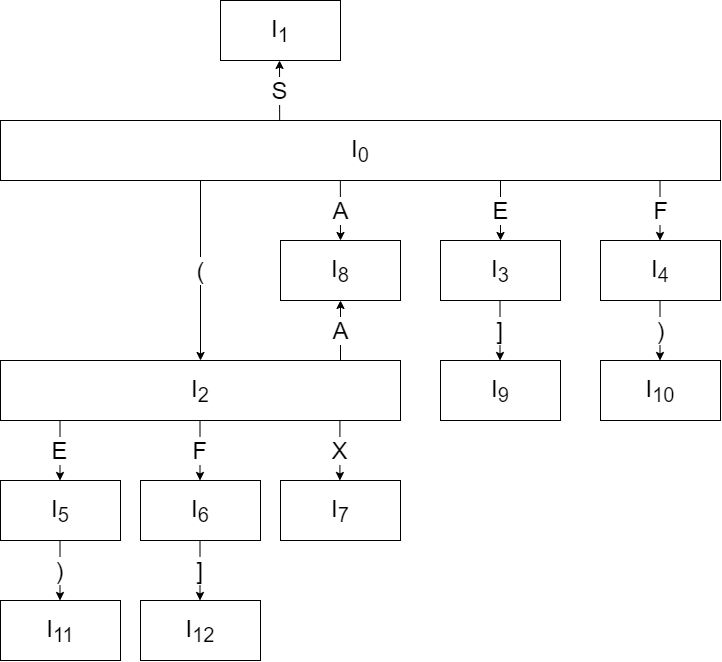
\includegraphics[width=10cm]{./01.png}
\end{figure}

\section{}
\begin{table}[H]
  \centering
  \begin{tabular}{|c||c|c|c|c|c|c|c|c|c|}\hline
       & \multicolumn{4}{c|}{action} & \multicolumn{5}{c|}{goto}                                                       \\\hline
       & (                          & ]                        & )                        & \#  & S & X & E & F & A \\\hline\hline
    0  & s2                          & r8                        & r8                        &     & 1 &   & 3 & 4 & 8 \\\hline
    1  &                             &                           &                           & acc &   &   &   &   &   \\\hline
    2  &                             & r8                        & r8                        &     &   & 7 & 5 & 6 & 8 \\\hline
    3  &                             & s9                        &                           &     &   &   &   &   &   \\\hline
    4  &                             &                           & s10                       &     &   &   &   &   &   \\\hline
    5  &                             &                           & s11                       &     &   &   &   &   &   \\\hline
    6  &                             & s12                       &                           &     &   &   &   &   &   \\\hline
    7  &                             &                           &                           & r1  &   &   &   &   &   \\\hline
    8  &                             & \begin{tabular}[c]{@{}c@{}}r6\\ r7\end{tabular} & \begin{tabular}[c]{@{}c@{}}r6\\ r7\end{tabular} &     &   &   &   &   &   \\\hline
    9  &                             &                           &                           & r2  &   &   &   &   &   \\\hline
    10 &                             &                           &                           & r3  &   &   &   &   &   \\\hline
    11 &                             &                           &                           & r4  &   &   &   &   &   \\\hline
    12 &                             &                           &                           & r5  &   &   &   &   &   \\\hline
  \end{tabular}
\end{table}

$I_8$で、Reduce/Reduce conflictが起こっているので、SLR(1)構文解析可能ではない。

\newpage
\section{}
\[I_0=[[S'\rightarrow \bullet S\#,\epsilon ],[S'\rightarrow \bullet (X,\#],[S\rightarrow \bullet E],\#],[S\rightarrow \bullet F),\#],[E\rightarrow \bullet A,]],[F\rightarrow \bullet A,)],[A\rightarrow \bullet ,]],[A\rightarrow \bullet ,)]]\]
\[I_1=[[S'\rightarrow S\bullet \#,\epsilon ]]\]
\[I_2=[[S\rightarrow (\bullet X,\#],[X\rightarrow \bullet E),\#],[X\rightarrow \bullet F],\#],[E\rightarrow \bullet A,)],[F\rightarrow \bullet A,]],[A\rightarrow \bullet ,]],[A\rightarrow \bullet ,)]]\]
\[I_3=[[S\rightarrow E\bullet ],\#]]\]
\[I_4=[[S\rightarrow F\bullet ),\#]]\]
\[I_5=[[E\rightarrow A\bullet ,]],[F\rightarrow A\bullet ,)]]\]
\[I_6=[[X\rightarrow E\bullet ),\#]]\]
\[I_7=[[X\rightarrow F\bullet ],\#]]\]
\[I_8=[[S\rightarrow (X\bullet ,\#]]\]
\[I_9=[[E\rightarrow A\bullet ,)],[F\rightarrow A\bullet ,]]]\]
\[I_{10}=[[S\rightarrow E]\bullet ,\#]]\]
\[I_{11}=[[S\rightarrow F)\bullet ,\#]]\]
\[I_{12}=[[X\rightarrow E)\bullet ,\#]]\]
\[I_{13}=[[X\rightarrow F]\bullet ,\#]]\]

\begin{figure}[H]
  \centering
  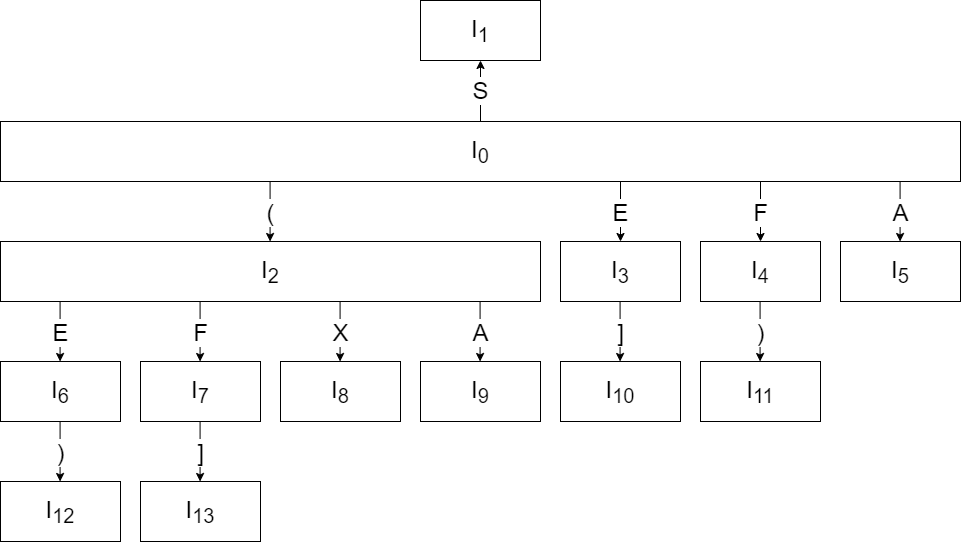
\includegraphics[width=10cm]{./02.png}
\end{figure}

\newpage
\section{}
\begin{table}[H]
  \centering
  \begin{tabular}{|c||c|c|c|c|c|c|c|c|c|}
    \hline
       & \multicolumn{4}{c|}{action} & \multicolumn{5}{c|}{goto}                                 \\ \hline
       & (                          & ]                        & )  & \#  & S & X & E & F & A \\ \hline\hline
    0  & s2                          & r8                        & r8  &     & 1 &   & 3 & 4 & 5 \\ \hline
    1  &                             &                           &     & acc &   & 8 & 6 & 7 & 9 \\ \hline
    2  &                             & r8                        & r8  &     &   &   &   &   &   \\ \hline
    3  &                             & s10                       &     &     &   &   &   &   &   \\ \hline
    4  &                             &                           & s11 &     &   &   &   &   &   \\ \hline
    5  &                             & r6                        & r7  &     &   &   &   &   &   \\ \hline
    6  & s12                         &                           &     &     &   &   &   &   &   \\ \hline
    7  &                             & s13                       &     &     &   &   &   &   &   \\ \hline
    8  &                             &                           &     & r1  &   &   &   &   &   \\ \hline
    9  &                             & r7                        & r6  &     &   &   &   &   &   \\ \hline
    10 &                             &                           &     & r2  &   &   &   &   &   \\ \hline
    11 &                             &                           &     & r3  &   &   &   &   &   \\ \hline
    12 &                             &                           &     & r4  &   &   &   &   &   \\ \hline
    13 &                             &                           &     & r5  &   &   &   &   &   \\ \hline
  \end{tabular}
\end{table}

衝突しないので、LR(1)構文解析可能ではない。

\end{document}
